\documentclass[a4paper, 11pt]{article}
\usepackage{geometry}
\usepackage{indentfirst}
\usepackage{setspace}
\usepackage{amsmath}
\usepackage{graphicx}
\usepackage{wrapfig}
\usepackage{caption}
\usepackage{indentfirst}
\setlength{\parindent}{20pt}
\usepackage{amssymb}
\usepackage{float}
\usepackage{subcaption}

\graphicspath{ {./images/} }
\geometry{left=2.5cm, right=2.5cm, top=2.5cm, bottom=2.5cm}

\begin{document}	
	\title{Exercise \# 3. Numerical Solution of the Poisson Problem. }
	\author{{\small Alexandre Rodrigues (2039952)}}
	\date{\today}
	
	\maketitle
		\section{Method}
			I will describe relevant steps of developing this implementation and respective theory.
			Based on the homework text I implemented each step in Matlab.
			
			\begin{enumerate}
				\item \textbf{Input files from specified mesh}: The user selects a mesh refinement level (0 to 4), all 3 files are loaded: \texttt{topol}, \texttt{bound} and \texttt{coord}.	
				\item \textbf{create pattern for the stiffness matrix}: 1st I created a range vector 1 to Ne, then place it 3 times in a matrix and convert the matrix to obtain the \texttt{row} vector $ row = [1,1,1,2,2,2,3,\ldots] $. The \texttt{col} vector is simply obtained by reshaping the \texttt{topol} as a column vector. Then we can compute the adjancy matrix as \texttt{A = sparse(row,col,1)} and finaly the pattern for the stifness matrix as \texttt{H = A' * A}.
				\item \textbf{Stifness matrix}:
				I created the function \texttt{[H, delta] = computeStiff(H, topol, coord)} to encapsulate all the following computations.
				It has the topology and coordinates matrixes as input as well as the H matrix with its pattern already defined before.
				Its outputs are the final H matrix and the \texttt{delta} vector with the surface measures of each element.
				Using a for loop for each element:
				3.1 - get coordinates of the 3 nodes that define the element, compute the surface measure for that element and save in the \texttt{delta} vector.
				3.2 - compute b,c (a is not needed): $\ldots$s
				3.3 - compute Hloc as $\ldots$ (Algorithm 3.3)
				\item  \textbf{Right hand size}
				Using a for loop:
				4.1 - get coords of the node;
				4.2 - find <elements that have that node as a vertex to get their surface measures
				$\ldots$
				4.3 - compute the rhs as $fxy * surfs/3 $
				\item \textbf{Boundary Conditions}
				As explained in the homework text we can simply change the diagonal value Hii.
				When susbititutiing Hii=Rmax I got a nonpositive pivot H matrix resulting in a error when computing the Choledsky factorization.
				The solution was to multiply Hii by Rmax instead of replacing it. \texttt{H(i,i) = Rmax*H(i,i)}.
				\item \textbf{Solve the Linear System}
				Using tolerance as 1e-8 and Matlab's PCG method.$\ldots$
				Jacobi preconditioner as \texttt{M = sparse(diag(diag(H)))}.
				Choledsky preconditioner as \texttt{L = ichol(H)}.
				Then we can call the PCG method to solve the linear system.
				I also recorded the solving computational time for comparison.
				Finally we can show the convergence plots as the semi logratimic plot of Residual Norm vs Iterations.
				\item \textbf{Error computation}
				Using a for loop to visit each node:
				7.1 - get the coordinates of the node;
				7.2 - compute the analytical solution as $u_a = x^2 + y^2 - x^2y^2 - 1$.
				7.3 - sum surface measures of each element that have this node as a vertex;
				7.4 - compute local error as $\ldots$
				7.5 - sum all local error and $ \epsilon $ will be its square root.	
			\end{enumerate}
			
	
		
		\section{Results}
		
			\subsection{Convergence Plots}
			
				$\ldots$
				
				\begin{figure}[H]
					\begin{subfigure}{.49\textwidth}
						\centering
						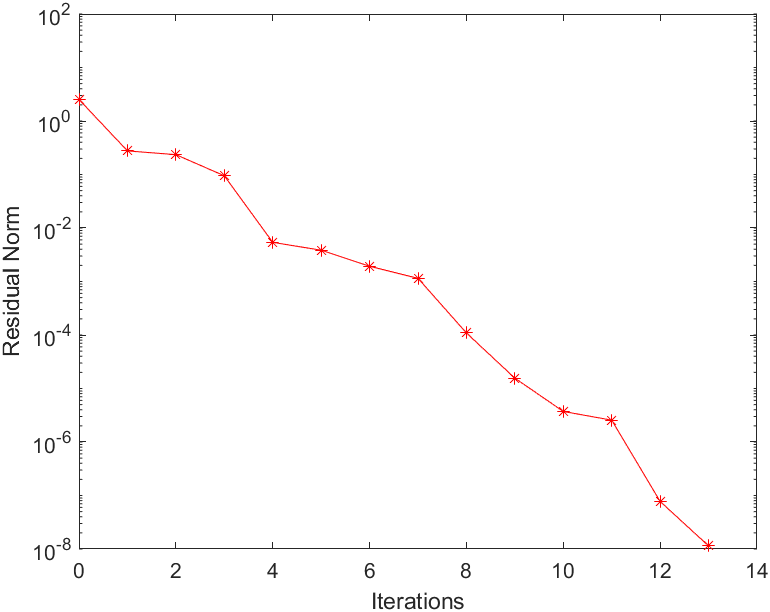
\includegraphics[width=.99\linewidth]{img0/J.png}  
						\caption{Jacobi}
						\label{fig:Jacobi_0}
					\end{subfigure}
					\begin{subfigure}{.49\textwidth}
						\centering
						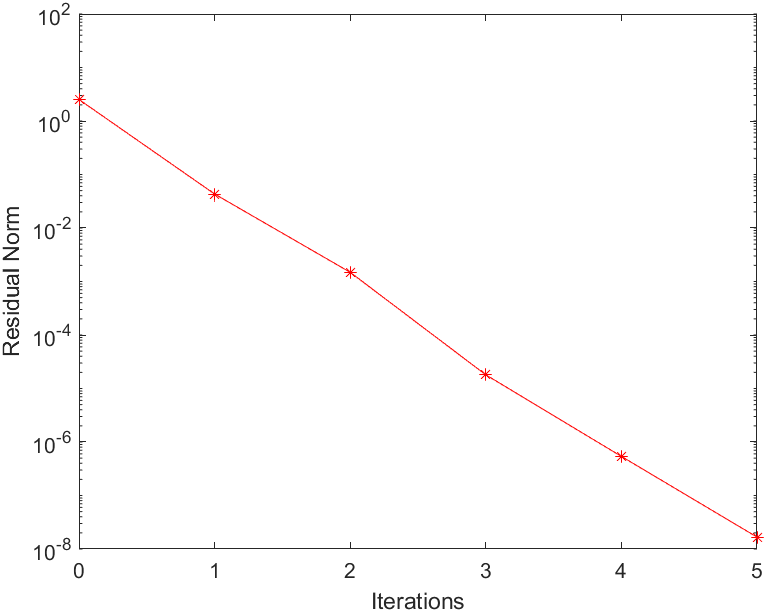
\includegraphics[width=.99\linewidth]{img0/C.png}  
						\caption{Choledsky}
						\label{fig:Chol_0}
					\end{subfigure}
					\caption{Convergence plots for level 0}
					\label{fig:fig0}
				\end{figure}
				
				\begin{figure}[H]
					\begin{subfigure}{.49\textwidth}
						\centering
						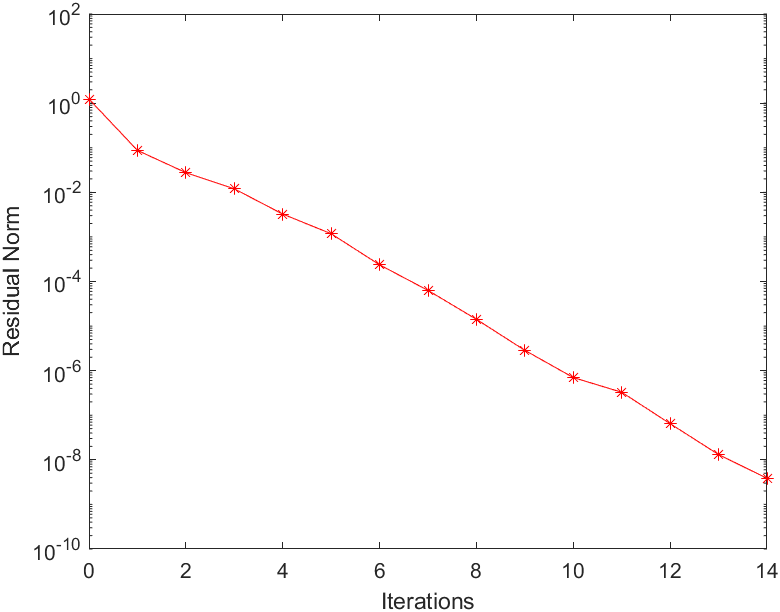
\includegraphics[width=.99\linewidth]{img1/J.png}  
						\caption{Jacobi}
						\label{fig:Jacobi_1}
					\end{subfigure}
					\begin{subfigure}{.49\textwidth}
						\centering
						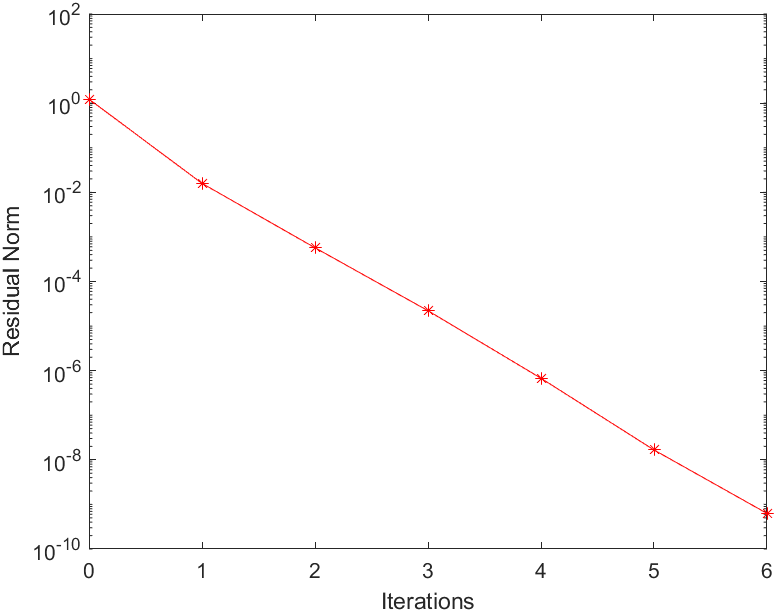
\includegraphics[width=.99\linewidth]{img1/C.png}  
						\caption{Choledsky}
						\label{fig:Chol_1}
					\end{subfigure}
					\caption{Convergence plots for level 1}
					\label{fig:fig1}
				\end{figure}
			
				\begin{figure}[H]
					\begin{subfigure}{.49\textwidth}
						\centering
						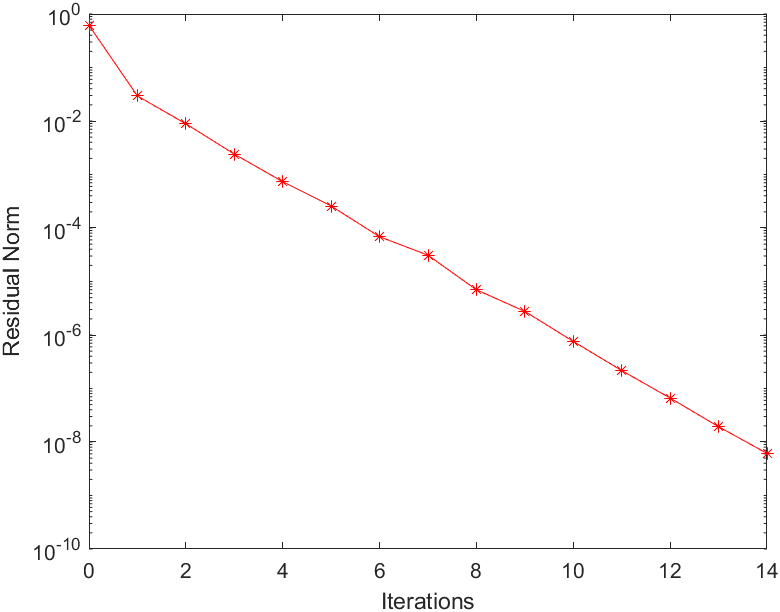
\includegraphics[width=.99\linewidth]{img2/J.png}  
						\caption{Jacobi}
						\label{fig:Jacobi_2}
					\end{subfigure}
					\begin{subfigure}{.49\textwidth}
						\centering
						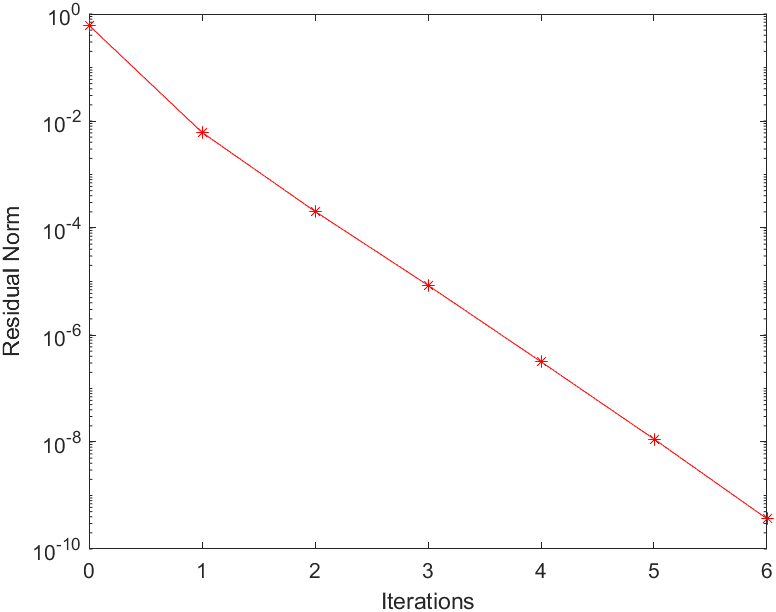
\includegraphics[width=.99\linewidth]{img2/C.png}  
						\caption{Choledsky}
						\label{fig:Chol_2}
					\end{subfigure}
					\caption{Convergence plots for level 2}
					\label{fig:fig2}
				\end{figure}
			
				\begin{figure}[H]
					\begin{subfigure}{.49\textwidth}
						\centering
						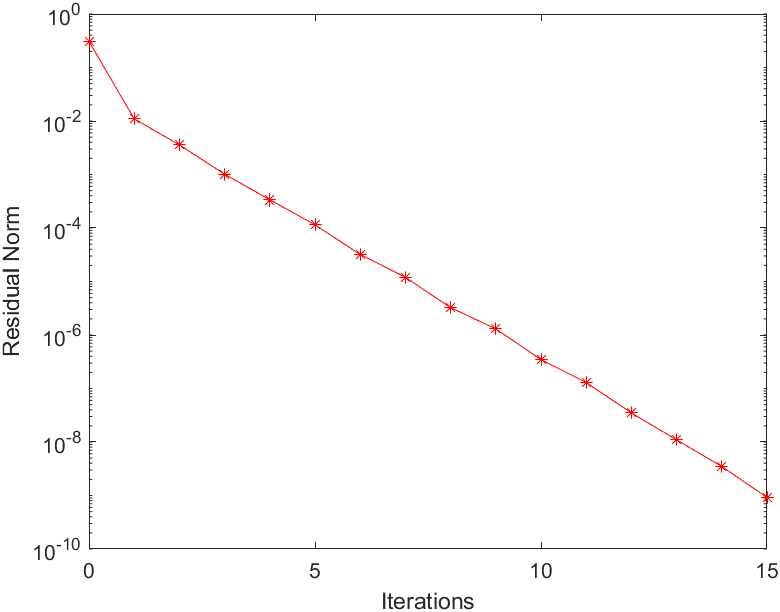
\includegraphics[width=.99\linewidth]{img3/J.png}  
						\caption{Jacobi}
						\label{fig:Jacobi_3}
					\end{subfigure}
					\begin{subfigure}{.49\textwidth}
						\centering
						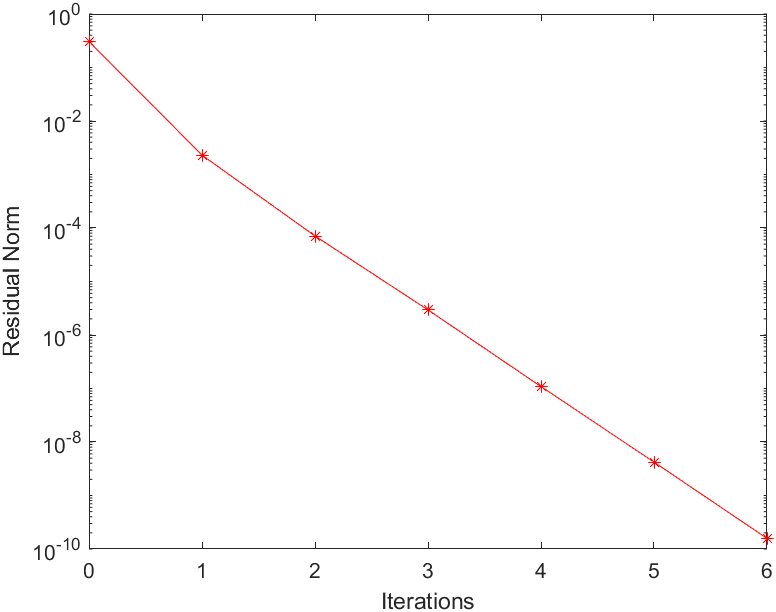
\includegraphics[width=.99\linewidth]{img3/C.png}  
						\caption{Choledsky}
						\label{fig:Chol_3}
					\end{subfigure}
					\caption{Convergence plots for level 3}
					\label{fig:fig3}
				\end{figure}
			
				\begin{figure}[H]
					\begin{subfigure}{.49\textwidth}
						\centering
						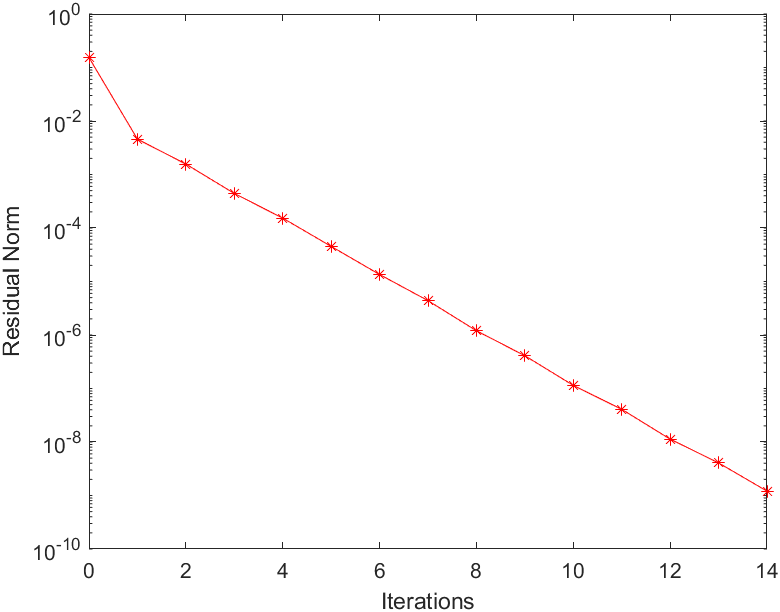
\includegraphics[width=.99\linewidth]{img4/J.png}  
						\caption{Jacobi}
						\label{fig:Jacobi_4}
					\end{subfigure}
					\begin{subfigure}{.49\textwidth}
						\centering
						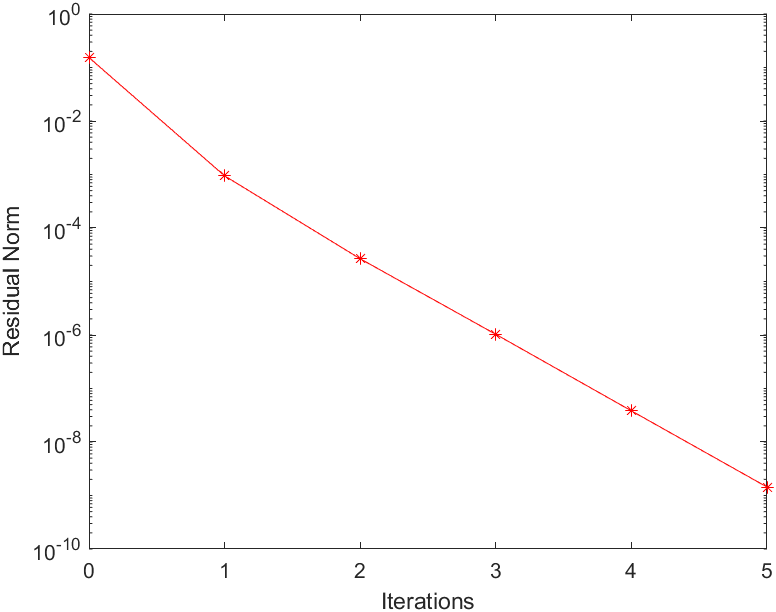
\includegraphics[width=.99\linewidth]{img4/C.png}  
						\caption{Choledsky}
						\label{fig:Chol_4}
					\end{subfigure}
					\caption{Convergence plots for level 4}
					\label{fig:fig4}
				\end{figure}
				
				There are clear differences in convergence when using the 2 preconditioners.
				The Choledsky preconditioner significantly improves convergence by reducing the number of iterations needed.
				There are no significant differences regarding the residual norms and between levels of refinement.
			
			\subsection{Epsilon}
				\begin{table}[H]
					\centering
%					\begin{tabular}{c|c|c}
%						\textbf{Level} 	& \textbf{$ \epsilon $} & \textbf{ Error Ratio}  \\ \hline
%						$ 0  $			& $ 0.9931 $ & N/A \\ \hline
%						$ 1  $			& $ 1.0231 $ & $ 1.0302 $ \\ \hline
%						$ 2  $			& $ 1.0217 $ & $ 0.9986 $ \\ \hline
%						$ 3  $			& $ 1.0190 $ & $ 0.9974 $ \\ \hline
%						$ 4  $			& $ 1.0176 $ & $ 0.9986 $ \\ 
%					\end{tabular}
					\begin{tabular}{c|c|c}
						\textbf{Level} 	& \textbf{$ \epsilon $} & \textbf{ Error Ratio}  \\ \hline
						$ 0  $			& $ 0.9931 $ 			& N/A \\ \hline
						$ 1  $			& $ 1.0508 $ 			& $ 1.0581 $ \\ \hline
						$ 2  $			& $ 1.0629 $ 			& $ 1.0115 $ \\ \hline
						$ 3  $			& $ 1.0657 $	 		& $ 1.0026 $ \\ \hline
						$ 4  $			& $ 1.0664 $ 			& $ 1.0007 $ \\ 
					\end{tabular}
					\caption{FEM Convergence table}
					\label{table:errors}
				\end{table}
				The $ \epsilon $ value slightly increases on each step of refinement....??
	
	
\end{document}



